\documentclass{beamer}

%--% Paquetes %----------------------------------%
\usepackage[spanish]{babel}
\usepackage[utf8]{inputenc}
\usepackage[T1]{fontenc}
\usepackage{graphicx}
\usepackage{hyperref}
\usepackage{courier}
\usepackage{listings}
\usepackage{xcolor}
\usepackage{blindtext}
\usepackage{scrextend}
\usepackage[document]{ragged2e}
\usepackage{multicol}
\usepackage{pgfgantt}
\usepackage{minted}
\usepackage{tikz}
\usepackage{longtable}
\usepackage{algorithm}
\usepackage[noend]{algpseudocode}
\usepackage{amsmath}
\usepackage{wrapfig,lipsum,booktabs}
%------------------------------------------------%

%En caso de que LaTeX separe las palabras con - de manera incorrecta, usar
%\hyphenation{deci-sión,e-xa-men, otras palabras....}
\hyphenation{o-cu-rrir}


\usetikzlibrary{positioning,fit,calc}

\makeatletter
\newcommand*{\MoveFitHeight}[1]{%
	\pgfmathsetlengthmacro\fit@inner@sep{%
		\pgfkeysvalueof{/pgf/inner xsep}%
	}%
	\pgfmathsetlengthmacro\fit@text@height{%
		\tikz@text@height
	}%
	\kern-\fit@inner@sep\relax
	\raisebox{\fit@text@height}[0pt][0pt]{#1}%
}
\makeatother

\newcommand{\algTitle}{\textbf{Algoritmo:} }

\newcommand{\bigO}[1]{$O({#1})$}

\usetheme{Berlin}
%\usecolortheme{beaver}

%--% Personal Info %-----------------------------%
\title{Segmentación y Paginación}
\author{Victor Tortolero, 24.569.609}
\institute{
	Sistemas Operativos, FACYT
}
\date{\today}
%------------------------------------------------%


\begin{document}
\setbeamertemplate{caption}{\raggedright\insertcaption\par}

\begin{frame}
	\titlepage

\end{frame}
\author{}


%---------------------------------------------------------------------------------%
\begin{frame}
\frametitle{Determinación del tamaño de la pagina}

\begin{itemize}
	\item Potencia de $2$, que varia entre $512$ bytes y $1$ GB por pagina.
	\item Depende del hardware, pero el sistema operativo puede jugar con su valor.
	\item Si es muy grande, ocurre fragmentación interna.
	\item Si es muy pequeña, los procesos tendrán muchas paginas.
\end{itemize}

\end{frame}


%---------------------------------------------------------------------------------%
\begin{frame}
	\frametitle{Tabla de páginas invertidas}
	
	\begin{itemize}
		\footnotesize
		\item Una entrada por cada marco.
		\item Reduce la cantidad de memoria necesaria para guardar cada tabla de paginas
		\item Incremente el tiempo de búsqueda de una pagina.
		\item Dificultad para implementar memoria compartida
	\end{itemize}
	
	\begin{figure}[H]
		\centering
		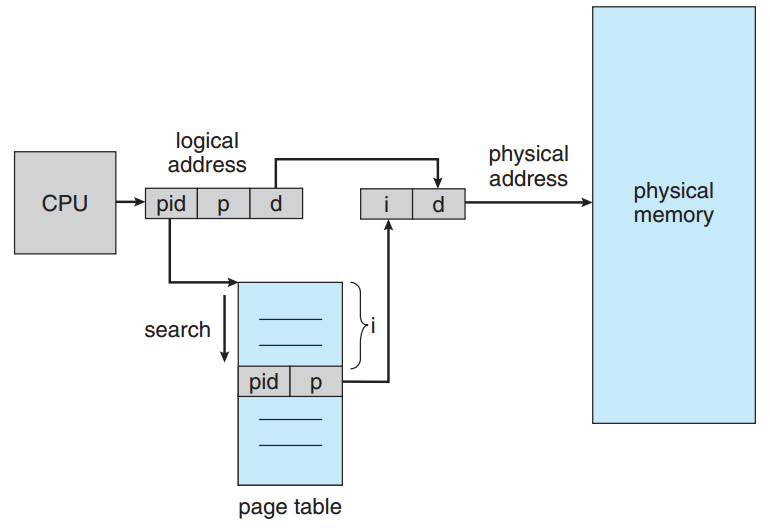
\includegraphics[scale=0.3]{img/pagina_invertida.png}
	\end{figure}
\end{frame}


%---------------------------------------------------------------------------------%
\begin{frame}
	\frametitle{Tabla de páginas invertidas}
	
	\begin{itemize}
		\item Las entradas de las tablas de niveles superiores apuntan a las inferiores sucesivamente.
		\item Las entradas de las tablas del ultimo nivel apuntan directamente a marcos de pagina
		\item Reduce el gasto de memoria.
		\item El numero de pagina se divide según el número de niveles.
	\end{itemize}
	
\end{frame}

\begin{frame}
	\frametitle{Tabla de páginas invertidas}
	
	\begin{figure}[H]
		\centering
		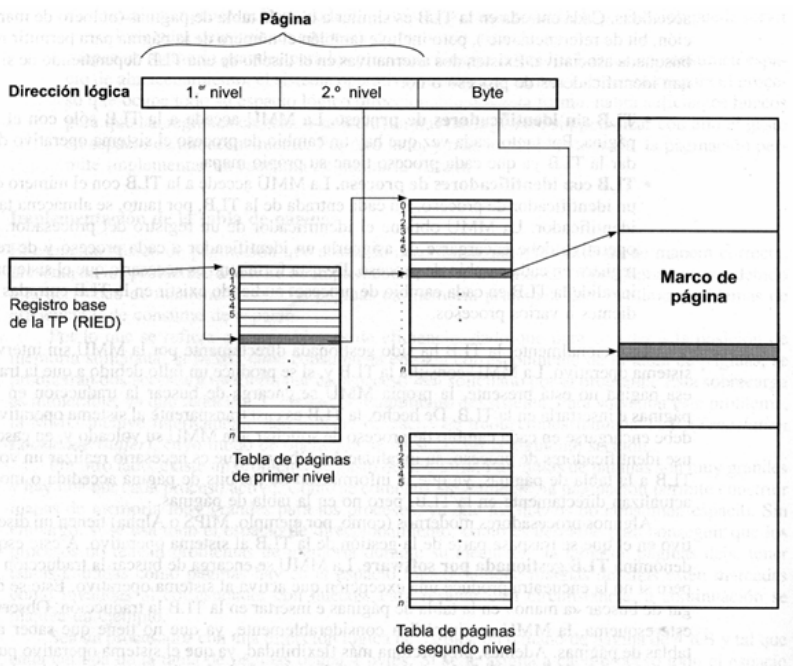
\includegraphics[scale=0.37]{img/paginacion_multi.png}
	\end{figure}
\end{frame}


%---------------------------------------------------------------------------------%
\begin{frame}
	\frametitle{Proteccion con paginacion}
	
	\begin{itemize}
		\item Se usan bits de protección.
		\item Bits para indicar cada tipo de acceso.
		\item Bit invalido-valido, cuando es valido la pagina asociada se encuentra en el espacio de direcciones lógicas del proceso, en caso contrario no se encuentra.
	\end{itemize}
\end{frame}

\begin{frame}
	\begin{figure}[H]
		\centering
		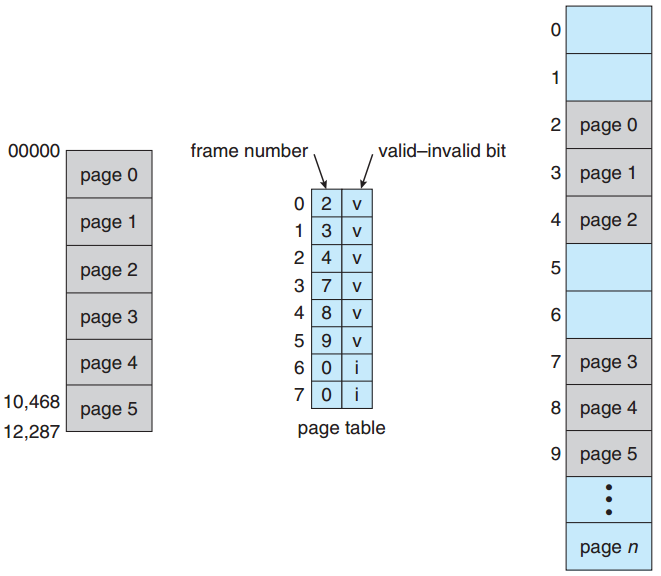
\includegraphics[scale=0.6]{img/paginacion_proteccion.png}
		\caption{Bit valido-invalido en una tabla de paginas}
	\end{figure}
\end{frame}


%---------------------------------------------------------------------------------%
\begin{frame}
	\frametitle{Proteccion con segmentación}
	
	\begin{itemize}
		\item Se usan bits de protección.
		\item Bits para indicar cada tipo de acceso.
		\item Bit invalido-valido, cuando es valido la pagina asociada se encuentra en el espacio de direcciones lógicas del proceso, en caso contrario no se encuentra.
	\end{itemize}
\end{frame}

\begin{frame}
	\begin{figure}[H]
		\centering
		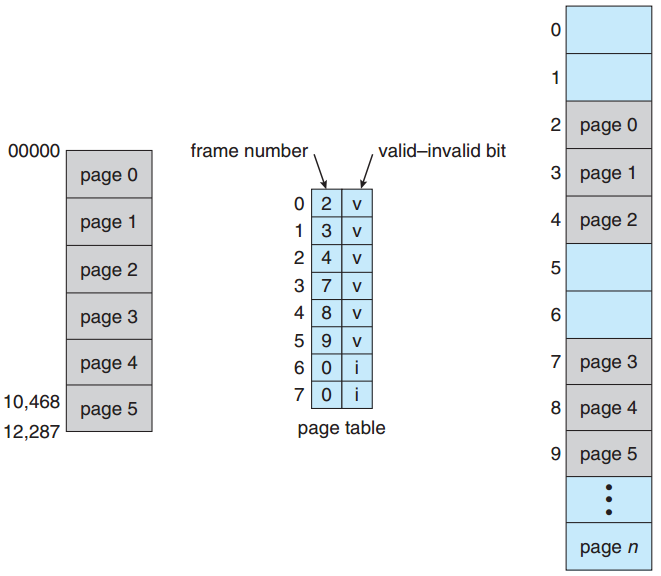
\includegraphics[scale=0.6]{img/paginacion_proteccion.png}
		\caption{Bit valido-invalido en una tabla de paginas}
	\end{figure}
\end{frame}


%---------------------------------------------------------------------------------%
\begin{frame}
	\frametitle{Comparticion con paginación}
	
	\begin{itemize}
		\item Se usan bits de protección.
		\item Bits para indicar cada tipo de acceso.
		\item Bit invalido-valido, cuando es valido la pagina asociada se encuentra en el espacio de direcciones lógicas del proceso, en caso contrario no se encuentra.
	\end{itemize}
\end{frame}


%---------------------------------------------------------------------------------%
\begin{frame}
	\frametitle{Comparticion con segmentación}
	
	\begin{itemize}
		\item Se usan bits de protección.
		\item Bits para indicar cada tipo de acceso.
		\item Bit invalido-valido, cuando es valido la pagina asociada se encuentra en el espacio de direcciones lógicas del proceso, en caso contrario no se encuentra.
	\end{itemize}
\end{frame}



\end{document}